%\chapter{Preliminaries}



\chapter{提案手法}

\section{問題設定}

そのような問題点を踏まえ,提案手法では複数の参照点を学習に利用する手法を導入した.従来手法の拡張で複数の参照点を考慮できるようにするためには,参照点と変位(座標系)のいずれかに複数の参照点の情報を保持する機構を導入する必要がある.そこで参照点の候補に各参照点間の重心位置を採用することによって,参照点に複数の参照点の位置情報を含めることができると考えた.また本研究では物体移動動作を初期状態に対する最終状態の決定と定義し,動作中のトラジェクタ軌跡に関しては考えていないため,学習モデルはより単純なガウスモデルを使用した.
重心位置を参照点として考慮した際,構成する参照点同士の位置関係に対応した相対位置を学習するために,重心位置を原点として重心を構成する参照点の向きに軸を取る座標系を考慮する必要がある.そのため,重心位置に対する変位にはその構成参照点の数分の座標系を追加生成する.

\section{提案手法}

\subsection{参照点}

従来手法で採用されていた各物体位置,トラジェクタの初期位置,画面中央に加えて,提案手法では新たに2つ以上の任意の物体間の重心位置を参照点に含めた.即ち環境中の$n$個の物体に対して,参照点は$2^{n}$個考慮する.

\subsection{変位}

従来手法で考慮されていた2つの変位に加えて,複数の物体を考慮した動作の学習を実現するために提案手法では以下の3種類が存在するとした.

	\begin{enumerate}
		\item 参照点を原点とし,常に一定の相対位置に遷移する
		\item 参照点を原点とし,トラジェクタの初期位置に応じて遷移先が変化する
		\item 複数の物体の位置関係に応じて遷移先が変化する
	\end{enumerate}
これら3種類の違いについてFig.\ref{figure:difference_displacement}で示す.
%%%%%%%%%%%%%%%%%%%%%%%%%%%%%%%%%%%%%%%%%%%%%%%%%%%%%%%%%%%%%%%%%%%%%%%%%%%%%%%%%%%%%%%%%%%%%%%%%%%%%%%
	\begin{figure}[t]
%中央ぞろえ
		\begin{center}
			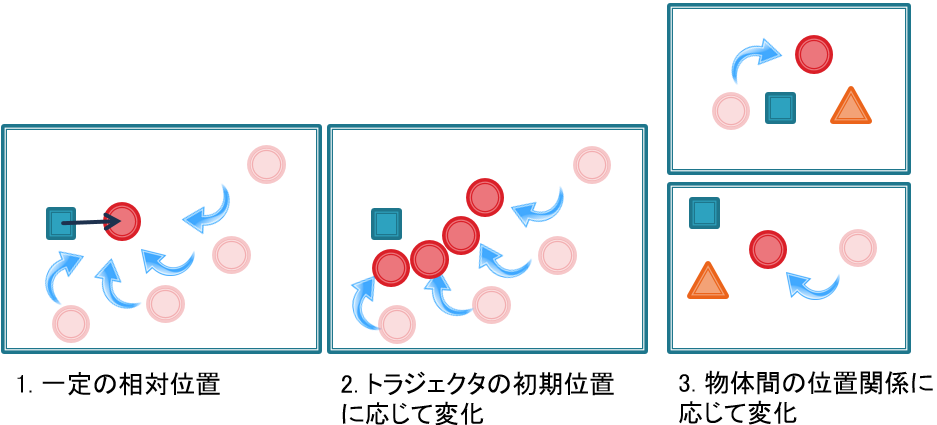
\includegraphics[width=14cm]{figure2.png} \\ %Teの基本として, \\ で緊急改行ができる.(今回の場合や行列などを除き,あまり使わない)
			\caption{参照点に対する遷移の違い}
			\label{figure:difference_displacement}
		\end{center}
	\end{figure}
%%%%%%%%%%%%%%%%%%%%%%%%%%%%%%%%%%%%%%%%%%%%%%%%%%%%%%%%%%%%%%%%%%%%%%%%%%%%%%%%%%%%%%%%%%%%%%%%%%%%%%%

3の例として,トラジェクタをある物体とある物体の間に動かすという動作などがあり,これは複数の物体を考慮した参照点の設定を行う必要がある.

\section{動作学習}

与えられた教示動作から,各観点のガウスモデルを学習する.まず教示動作の目標位置の,各参照点を原点とした相対位置を求め,各座標系ごとに座標変換,正規化を行う.それにより得たベクトル$v$を用いて,各ガウスモデルの平均$μ$,2乗平均$Q$,分散$σ$を以下のように更新する.

\[
	μ  \leftarrow \frac{N}{N+1}μ+\frac{1}{N+1}v
\]
\[
	Q  \leftarrow \frac{N}{N+1}Q+\frac{1}{N+1}v^2	
\]
\[
	σ  \leftarrow Q - μ^2
\]

動作学習のアルゴリズムの詳細については付録\ref{appendix3}に示す.


\section{動作再現}

教示動作から学習された各観点における確率モデルを用いて,異なる初期環境での動作再現を行う.まず学習された各観点のガウスモデルのうち最も分散の小さいものを探索する.分散が小さいとは教示動作がその観点に対して常に類似した目標位置に遷移していたことを意味し,教示者が意図した観点である可能性が高いと考えられる.選択された観点のガウスモデルの平均を,その観点と再現時の初期環境に応じた正規化と座標変換の逆関数を計算し,初期環境における参照点の位置に平行移動することで再現動作のトラジェクタの目標位置を推定する.
Fig.\ref{figure:learning_and_reproduction_model}に,提案手法における動作学習と動作再現の模式図を示す.
また付録\ref{appendix3}に,動作再現のアルゴリズムの詳細を示す.
%%%%%%%%%%%%%%%%%%%%%%%%%%%%%%%%%%%%%%%%%%%%%%%%%%%%%%%%%%%%%%%%%%%%%%%%%%%%%%%%%%%%%%%%%%%%%%%%%%%%%%%
	\begin{figure}[h]
%中央ぞろえ
		\begin{center}
			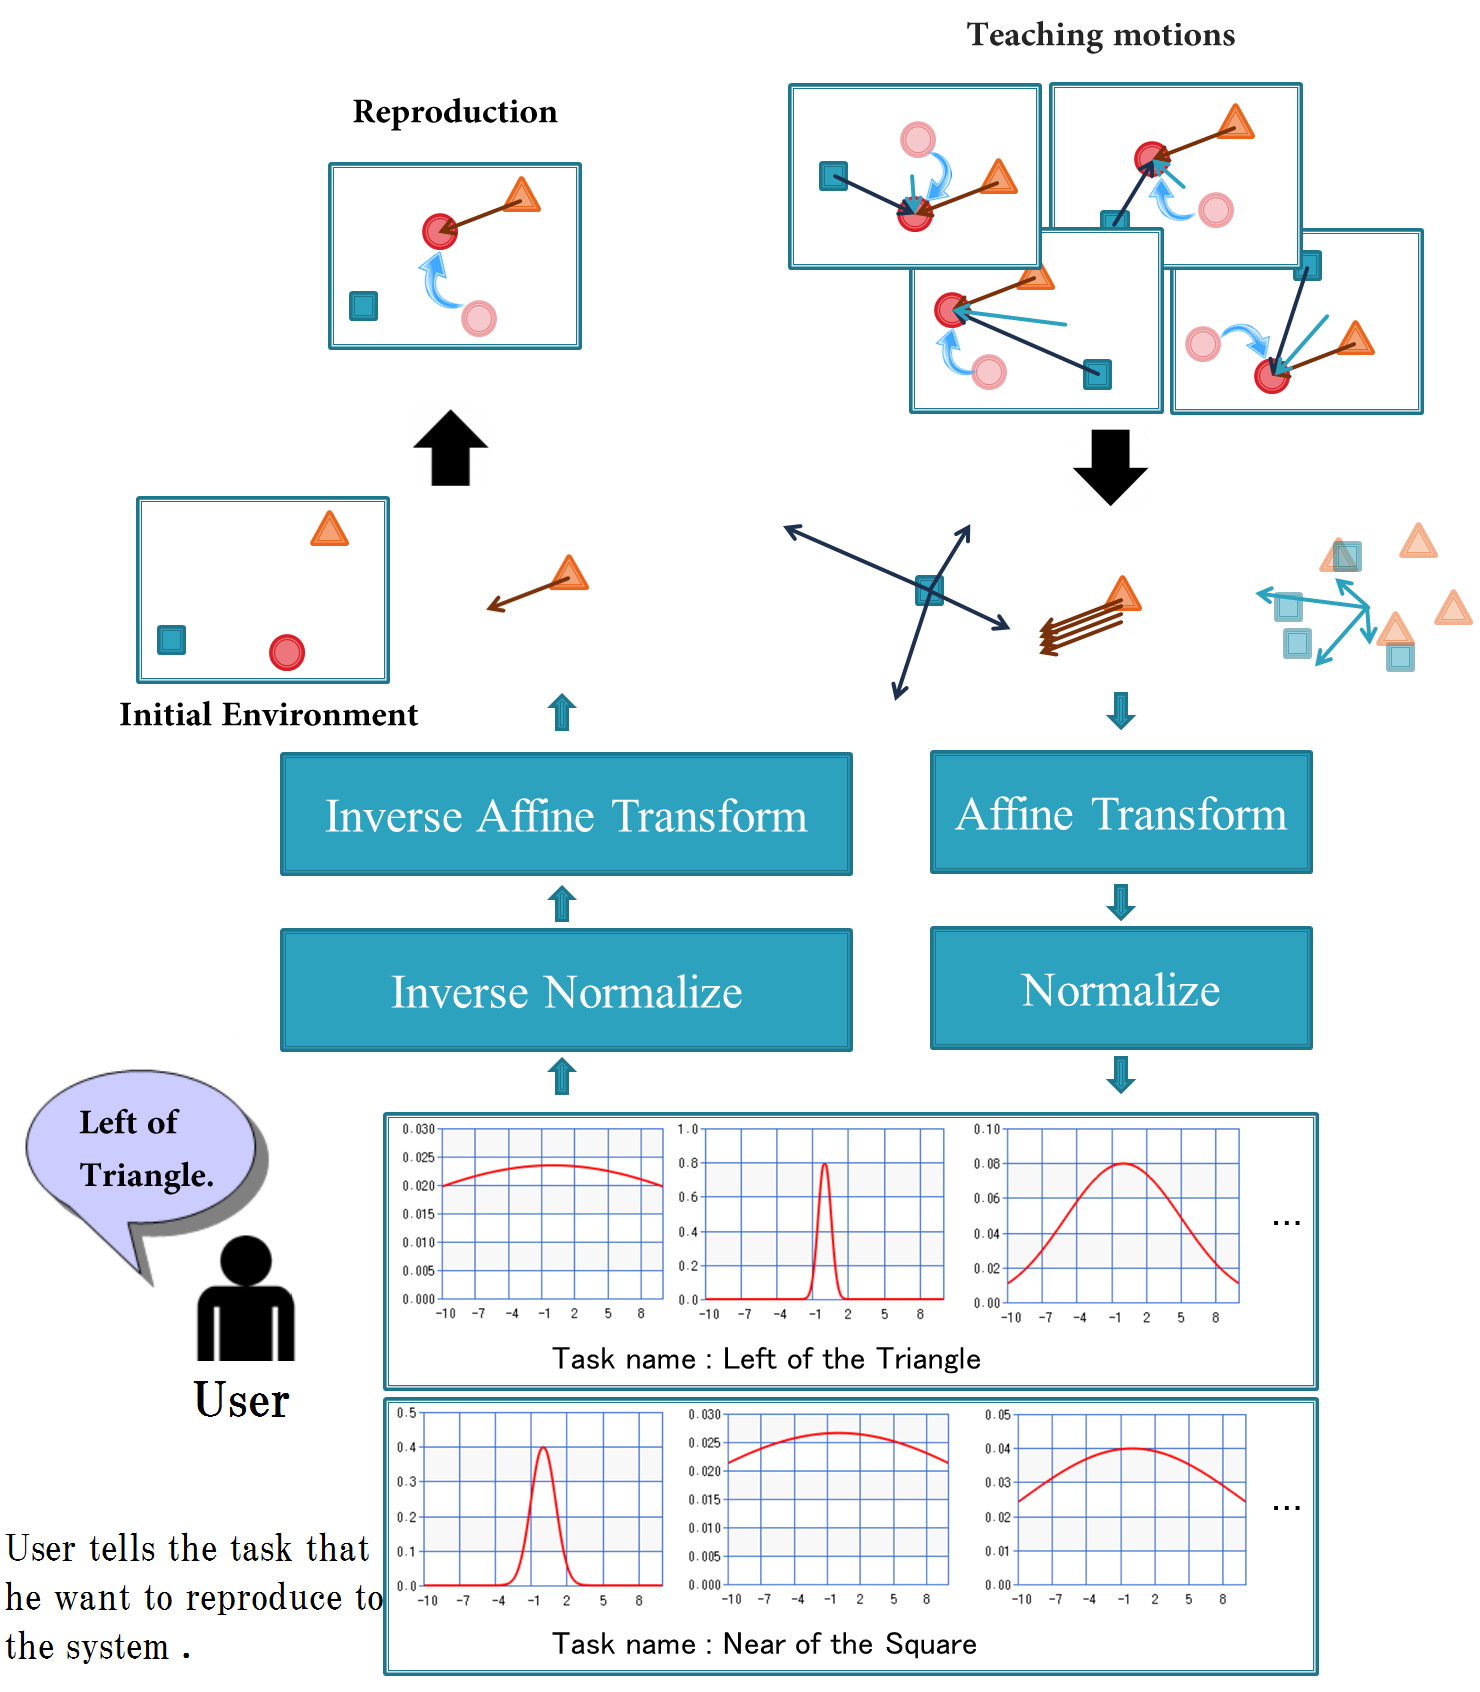
\includegraphics[width=12cm]{chart9.png} \\ %Teの基本として, \\ で緊急改行ができる.(今回の場合や行列などを除き,あまり使わない)
			\caption{動作学習と動作再現}
			\label{figure:learning_and_reproduction_model}
		\end{center}
	\end{figure}
%%%%%%%%%%%%%%%%%%%%%%%%%%%%%%%%%%%%%%%%%%%%%%%%%%%%%%%%%%%%%%%%%%%%%%%%%%%%%%%%%%%%%%%%%%%%%%%%%%%%%%%

\section{動作識別}

モデルが学習された各動作から例示動作の生起確率を計算することで,例示動作が既学習動作のうちいずれであるかを識別することが可能である.まず各動作において学習されたガウスモデルのうち分散が最小である観点を選択する.選択された観点のガウスモデルから,例示動作の目標位置が生起される確率をそれぞれ求め,生起確率が最大となるガウスモデルを持つ動作を識別結果とする.
Fig.\ref{figure:identification_model}に,提案手法における動作識別の模式図を示す.
また付録\ref{appendix3}に,動作識別のアルゴリズムの詳細を示す.
%%%%%%%%%%%%%%%%%%%%%%%%%%%%%%%%%%%%%%%%%%%%%%%%%%%%%%%%%%%%%%%%%%%%%%%%%%%%%%%%%%%%%%%%%%%%%%%%%%%%%%%
	\begin{figure}[h]
%中央ぞろえ
		\begin{center}
			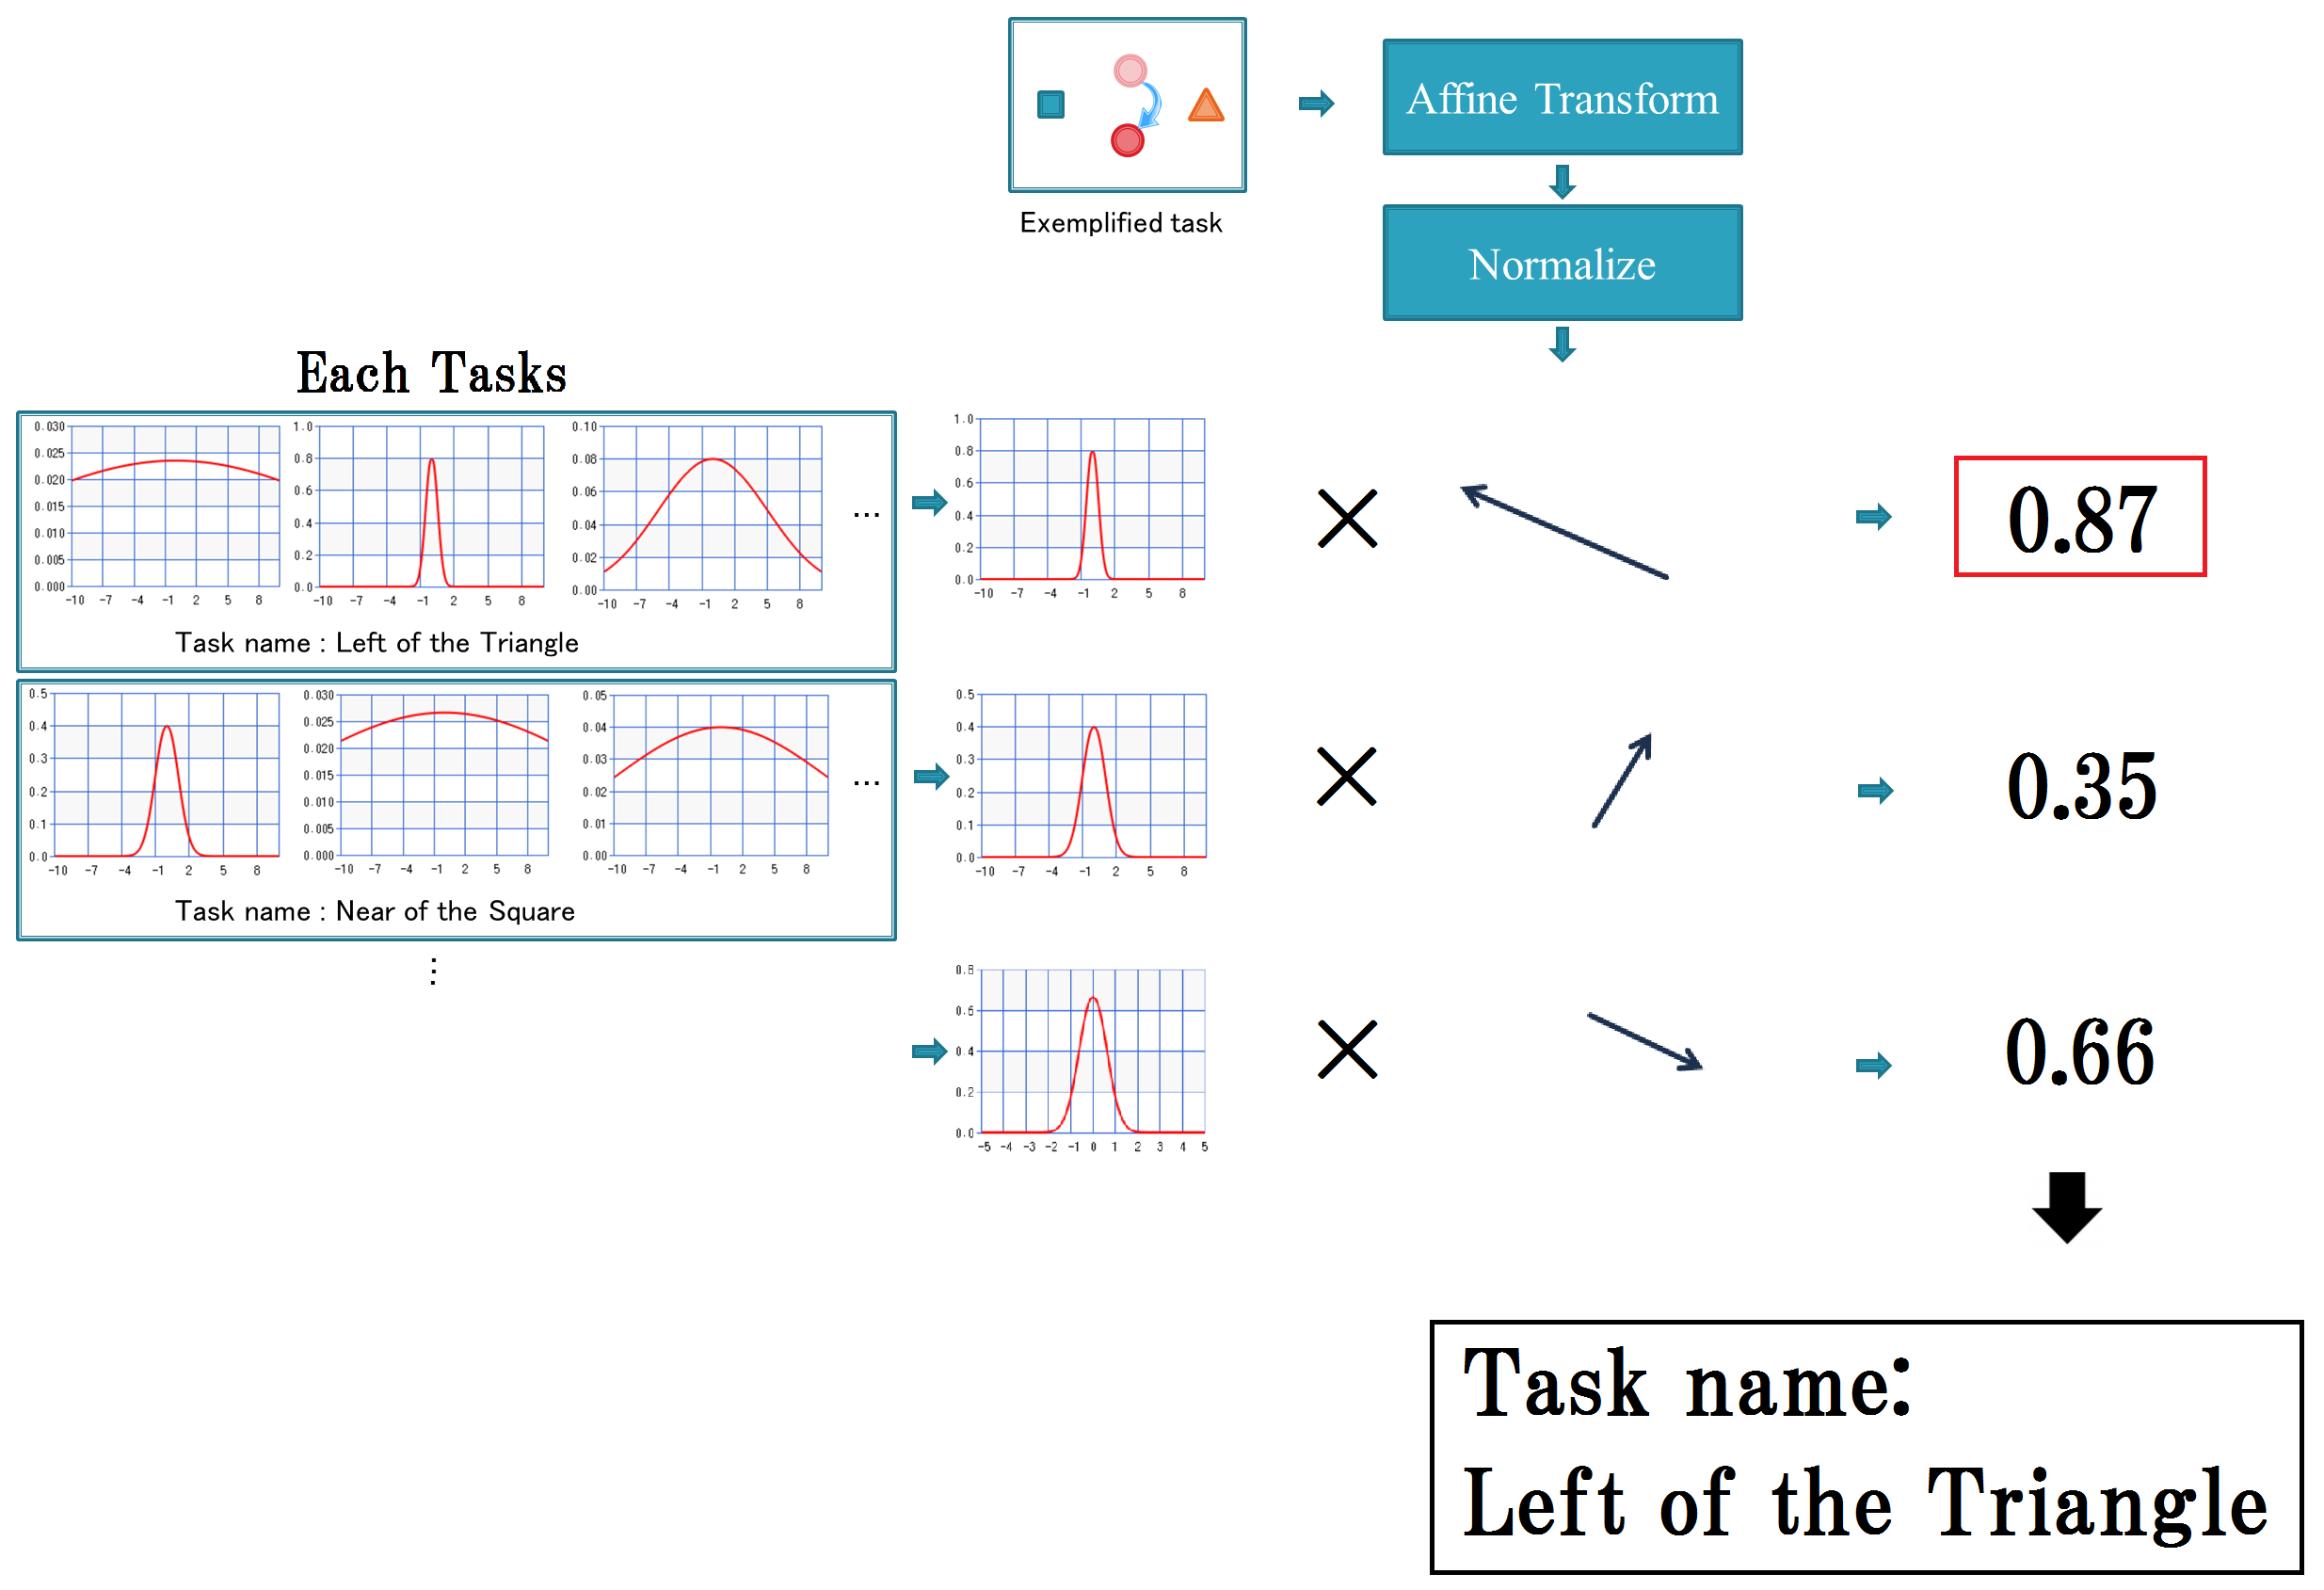
\includegraphics[width=14cm]{chart10.png} \\ %Teの基本として, \\ で緊急改行ができる.(今回の場合や行列などを除き,あまり使わない)
			\caption{動作識別}
			\label{figure:identification_model}
		\end{center}
	\end{figure}
%%%%%%%%%%%%%%%%%%%%%%%%%%%%%%%%%%%%%%%%%%%%%%%%%%%%%%%%%%%%%%%%%%%%%%%%%%%%%%%%%%%%%%%%%%%%%%%%%%%%%%%
